\section{Results}
\label{sec:results}

As discussed in section \ref{sec:methodology}, Monte Carlo simulations for 1D
Ising model were performed for different lattice sizes and temperatures. These
simulations generated configurations of the system at each montecarlo step.
These configurations were used to calculate the energy and magnetization of the
system. We used these values to calculate the autocorrelation time of the
magnetization as shown in figure \ref{fig:acf_mag}. 

\begin{figure}[ht]
    \centering
    \begin{subfigure}{0.45\textwidth}
        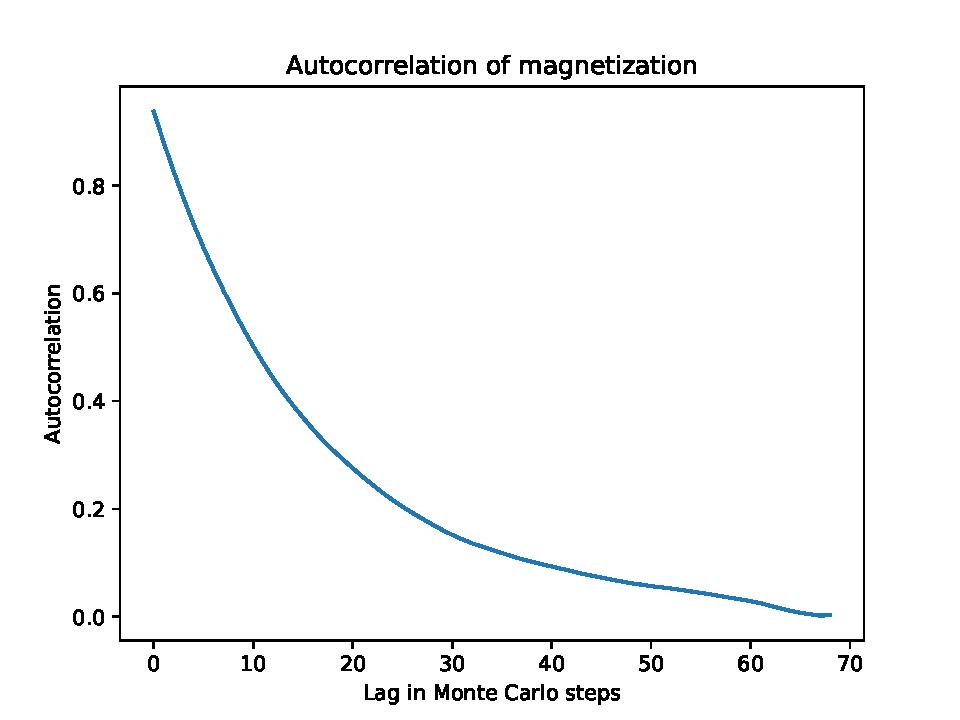
\includegraphics[width=\textwidth]{../plots/acf_mag.pdf}
        \caption{Exponentially decaying autocorrelation function for magnetization.}
        \label{fig:acf_mag}
    \end{subfigure}
    \hfill
    \begin{subfigure}{0.45\textwidth}
        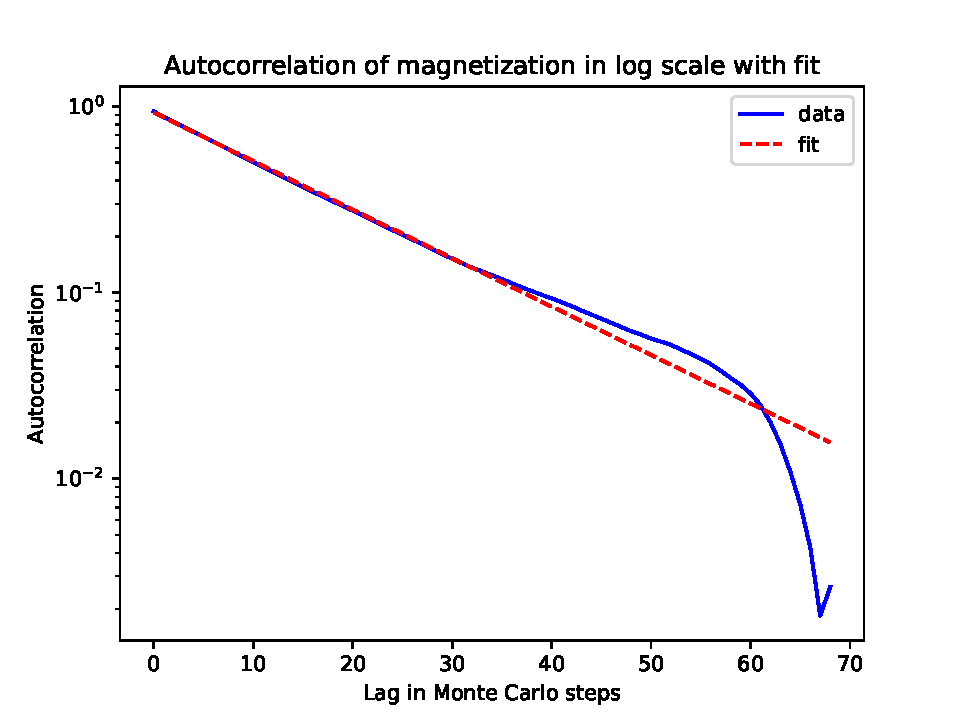
\includegraphics[width=\textwidth]{../plots/acf_mag_fit.pdf}
        \caption{Fit of an exponential function to the autocorrelation function on a log scale.}
        \label{fig:acf_mag_fit}
    \end{subfigure}
    \caption{Autocorrelation function for magnetization.}
\end{figure}

